% Options for packages loaded elsewhere
\PassOptionsToPackage{unicode}{hyperref}
\PassOptionsToPackage{hyphens}{url}
%
\documentclass[
]{article}
\usepackage{amsmath,amssymb}
\usepackage{lmodern}
\usepackage{ifxetex,ifluatex}
\ifnum 0\ifxetex 1\fi\ifluatex 1\fi=0 % if pdftex
  \usepackage[T1]{fontenc}
  \usepackage[utf8]{inputenc}
  \usepackage{textcomp} % provide euro and other symbols
\else % if luatex or xetex
  \usepackage{unicode-math}
  \defaultfontfeatures{Scale=MatchLowercase}
  \defaultfontfeatures[\rmfamily]{Ligatures=TeX,Scale=1}
\fi
% Use upquote if available, for straight quotes in verbatim environments
\IfFileExists{upquote.sty}{\usepackage{upquote}}{}
\IfFileExists{microtype.sty}{% use microtype if available
  \usepackage[]{microtype}
  \UseMicrotypeSet[protrusion]{basicmath} % disable protrusion for tt fonts
}{}
\makeatletter
\@ifundefined{KOMAClassName}{% if non-KOMA class
  \IfFileExists{parskip.sty}{%
    \usepackage{parskip}
  }{% else
    \setlength{\parindent}{0pt}
    \setlength{\parskip}{6pt plus 2pt minus 1pt}}
}{% if KOMA class
  \KOMAoptions{parskip=half}}
\makeatother
\usepackage{xcolor}
\IfFileExists{xurl.sty}{\usepackage{xurl}}{} % add URL line breaks if available
\IfFileExists{bookmark.sty}{\usepackage{bookmark}}{\usepackage{hyperref}}
\hypersetup{
  pdftitle={Codebook bundeslaendeR Election Data},
  pdfauthor={Robert Stelzle},
  hidelinks,
  pdfcreator={LaTeX via pandoc}}
\urlstyle{same} % disable monospaced font for URLs
\usepackage[margin=1in]{geometry}
\usepackage{graphicx}
\makeatletter
\def\maxwidth{\ifdim\Gin@nat@width>\linewidth\linewidth\else\Gin@nat@width\fi}
\def\maxheight{\ifdim\Gin@nat@height>\textheight\textheight\else\Gin@nat@height\fi}
\makeatother
% Scale images if necessary, so that they will not overflow the page
% margins by default, and it is still possible to overwrite the defaults
% using explicit options in \includegraphics[width, height, ...]{}
\setkeys{Gin}{width=\maxwidth,height=\maxheight,keepaspectratio}
% Set default figure placement to htbp
\makeatletter
\def\fps@figure{htbp}
\makeatother
\setlength{\emergencystretch}{3em} % prevent overfull lines
\providecommand{\tightlist}{%
  \setlength{\itemsep}{0pt}\setlength{\parskip}{0pt}}
\setcounter{secnumdepth}{-\maxdimen} % remove section numbering
\usepackage{longtable}
\usepackage{float}
\usepackage{graphicx}
\usepackage{booktabs}
\usepackage{longtable}
\usepackage{array}
\usepackage{multirow}
\usepackage{wrapfig}
\usepackage{float}
\usepackage{colortbl}
\usepackage{pdflscape}
\usepackage{tabu}
\usepackage{threeparttable}
\usepackage{threeparttablex}
\usepackage[normalem]{ulem}
\usepackage{makecell}
\usepackage{xcolor}
\ifluatex
  \usepackage{selnolig}  % disable illegal ligatures
\fi

\title{Codebook bundeslaendeR Election Data}
\author{Robert Stelzle}
\date{15 1 2022}

\begin{document}
\maketitle

\hypertarget{ltw_election_results}{%
\subsection{\texorpdfstring{\texttt{ltw\_election\_results}}{ltw\_election\_results}}\label{ltw_election_results}}

\texttt{bundeslaendeR::ltw\_election\_results} returns data frame
(tibble if the tibble package is loaded) containing one row per
contesting party per election.

Most election results data are provided by the Bundeswahlleiter. A
machine-readable version of the Bundeswahlleiter's compiled data
contained in the -periodically published- pdf available here
(\url{https://www.bundeswahlleiter.de/service/landtagswahlen.html}) was
kindly provided to me. Election data outside the timeframe covered by
Bundeswahlleiter's data provided to me was collected from the states'
local election authorities' (Landeswahlleiter) websites. More
information on parties and the continuity of parties under different
labels was collected by me.

The Bundeswahlleiter's election data in many cases contains differing
names for the same party. Both between states (eg. ``Christlich
Demokratische Union Deutschlands'' vs.~``Christlich Demokratische Union
Deutschlands in Niedersachsen'') as well as within states between
elections -in many cases due to parties being renamed- (``BÜNDNIS 90/DIE
GRÜNEN, Landesverband Hamburg, Grün-Alternative Liste'' vs.~``BÜNDNIS
90/DIE GRÜNEN, Landesverband Hamburg''). Efforts were made to reconcile
both of these inconsistencies by adding two new, harmonized variables
identifying parties (\texttt{partyname\_short} and \texttt{partyname}).
This harmonized party identifier also covers merging of parties. The
partyname given to the resulting party (eg. ``Linke'', ``Grüne'') is
given to the largest of the preceding parties contesting an election
unless a smaller party joined a government following the election. The
original names provided by the Bundeswahlleiter (and Landeswahlleiters
in elections after June 2021) are still available
(\texttt{partyname\_short\_bundeswahlleiter} and
\texttt{partyname\_bundeswahlleiter}).

\newpage

\hypertarget{variables}{%
\section{Variables}\label{variables}}

\begin{longtable}{p{3.2cm}| p{11cm}}
\texttt{state} &\textbf{State Abbreviation}\newline 
ISO 3166-2:DE-code of the state;
           including BA for the former state of Baden, WH for the former state
           of Württemberg-Hohenzollern and WB for the former state of
           Württemberg-Baden.
\end{longtable}

\begin{longtable}{p{3.2cm}| p{11cm}}
\texttt{nuts1} &\textbf{NUTS1 Code of State}\newline 
NUTS1 code of state. NA for former states Baden, Württemberg-Baden, Württemberg-Hohenzollern.
\end{longtable}

\begin{longtable}{p{3.2cm}| p{11cm}}
\texttt{state\_name\_de} &\textbf{German Name of State}\newline 
German name of the state.
\end{longtable}

\begin{longtable}{p{3.2cm}| p{11cm}}
\texttt{state\_name\_en} &\textbf{English Name of State.}\newline 
English name of the state.
\end{longtable}

\begin{table}

\caption{\label{tab:state_variables_table}Overview of state level variables}
\centering
\begin{tabular}[t]{llllr}
\toprule
state & nuts1 & state\_name\_de & state\_name\_en & n\\
\midrule
BA & NA & ehemaliges Land Baden & former state Baden & 4\\
BB & DE4 & Brandenburg & Brandenburg & 84\\
BE & DE3 & Berlin & Berlin & 245\\
BW & DE1 & Baden-Württemberg & Baden-Württemberg & 230\\
BY & DE2 & Bayern & Bavaria & 209\\
\addlinespace
HB & DE5 & Bremen & Bremen & 193\\
HE & DE7 & Hessen & Hesse & 224\\
HH & DE6 & Hamburg & Hamburg & 257\\
MV & DE8 & Mecklenburg-Vorpommern & Mecklenburg-Vorpommern & 128\\
NI & DE9 & Niedersachsen & Lower-Saxony & 205\\
\addlinespace
NW & DEA & Nordrhein-Westfalen & North Rhine-Westphalia & 267\\
RP & DEB & Rheinland-Pfalz & Rhineland-Palatine & 160\\
SH & DEF & Schleswig-Holstein & Schleswig-Holstein & 189\\
SL & DEC & Saarland & Saarland & 131\\
SN & DED & Sachsen & Saxony & 98\\
\addlinespace
ST & DEE & Sachsen-Anhalt & Saxony-Anhalt & 117\\
TH & DEG & Thüringen & Thuringia & 89\\
WB & NA & ehemaliges Land Württemberg-Baden & former state Württemberg-Baden & 9\\
WH & NA & ehemaliges Land Württemberg-Hohenzollern & former state Württemberg-Hohenzollern & 4\\
\bottomrule
\end{tabular}
\end{table}

\begin{longtable}{p{3.2cm}| p{11cm}}
\texttt{state\_election\_
term} &\textbf{Election Term of State}\newline 
Election term in the state. Counts up from 1.



\hspace*{.25cm}
\begin{minipage}[t]{\linewidth }
\vspace{0pt}
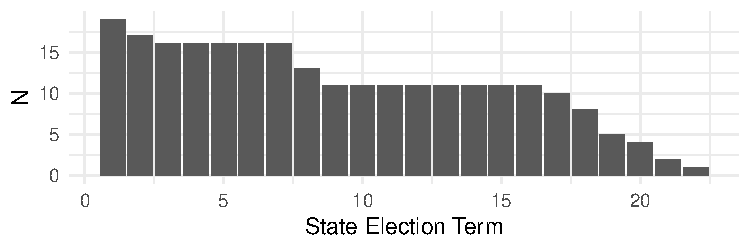
\includegraphics[width = \linewidth]{cbelec/electiontermplot.pdf}
\end{minipage}





\end{longtable}

\begin{longtable}{p{3.2cm}| p{11cm}}
\texttt{election\_date} &\textbf{Election Date}\newline 
Date of the election.  ISO 8601 or R-Date format.

\hspace*{.25cm}
\begin{minipage}[t]{\linewidth }
\vspace{0pt}
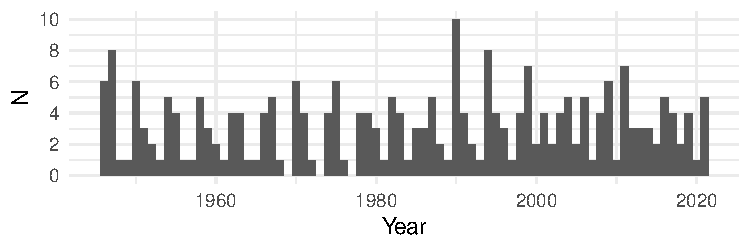
\includegraphics[width = \linewidth]{cbelec/electiondatesplot.pdf}
\end{minipage}


\end{longtable}

\begin{longtable}{p{3.2cm}| p{11cm}}
\texttt{election\_id\_
bundeswahlleiter} &\textbf{Election ID Bundeswahlleiter}\newline 
Specific election\_id as denoted by the Bundeswahlleiter. Note that BA, WH and WH are named as BW and the number counts down. NA for cases taken from Landeswahlleiters (ie elections after ST 2021).
\end{longtable}

\begin{longtable}{p{3.2cm}| p{11cm}}
\texttt{election\_remarks\_
bundeswahlleiter} &\textbf{Election Remarks Bundeswahlleiter}\newline 
Remarks on the election as given by the Bundeswahlleiter.
\end{longtable}

\begin{longtable}{p{3.2cm}| p{11cm}}
\texttt{electorate} &\textbf{Size of the Electorate}\newline 
Number of eligible voters. For more totals also see the last three columns.

\hspace*{.25cm}
\begin{minipage}[t]{\linewidth }
\vspace{0pt}
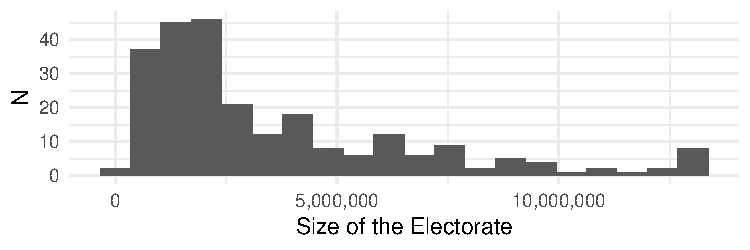
\includegraphics[width = \linewidth]{cbelec/electorateplot.pdf}
\end{minipage}


\end{longtable}

\begin{longtable}{p{3.2cm}| p{11cm}}
\texttt{number\_of\_voters} &\textbf{Number of Voters}\newline 
Number of voters turning out. For more totals also see the last three columns.

\hspace*{.25cm}
\begin{minipage}[t]{\linewidth }
\vspace{0pt}
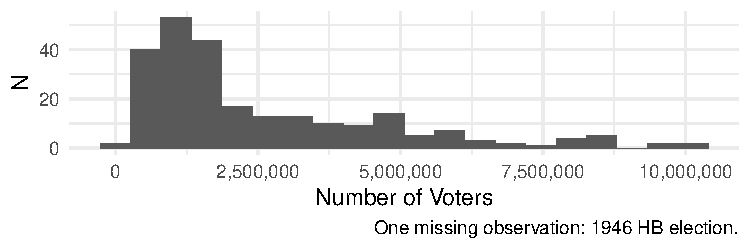
\includegraphics[width = \linewidth]{cbelec/nvotersplot.pdf}
\end{minipage}


\end{longtable}

\begin{longtable}{p{3.2cm}| p{11cm}}
\texttt{turnout} &\textbf{Turnout}\newline 
Turnout. Share of eligible voters turning out.

\hspace*{.25cm}
\begin{minipage}[t]{\linewidth }
\vspace{0pt}
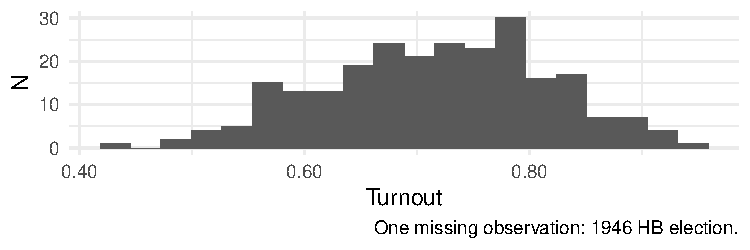
\includegraphics[width = \linewidth]{cbelec/turnoutplot.pdf}
\end{minipage}


\end{longtable}

\begin{longtable}{p{3.2cm}| p{11cm}}
\texttt{valid\_votes} &\textbf{Valid Votes}\newline 
Number of valid votes. Does not have to be equal to the number of ballots cast, as sometimes a ballot contains multiple votes! For more totals also see the last three columns.

\hspace*{.25cm}
\begin{minipage}[t]{\linewidth }
\vspace{0pt}
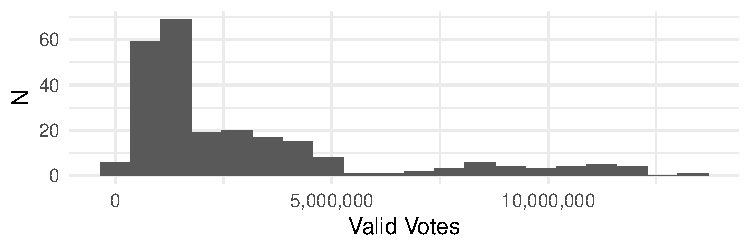
\includegraphics[width = \linewidth]{cbelec/validvoteplot.pdf}
\end{minipage}


\end{longtable}

\begin{longtable}{p{3.2cm}| p{11cm}}
\texttt{total\_seats\_
parliament} &\textbf{Total Seats in Parliament}\newline 
Total number of members of the newly elected Landtag.

\hspace*{.25cm}
\begin{minipage}[t]{\linewidth }
\vspace{0pt}
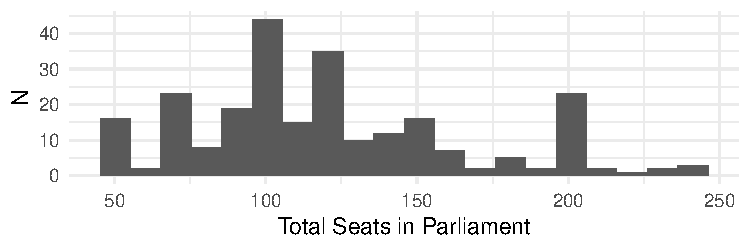
\includegraphics[width = \linewidth]{cbelec/tseatsparlplot.pdf}
\end{minipage}


\end{longtable}

\begin{longtable}{p{3.2cm}| p{11cm}}
\texttt{female\_party\_
seats\_available} &\textbf{Number of female MdLs available per party}\newline 
Denotes whether information on the no. of female members of the Landtag per party is available for this election. Note that for parties not elected to the new Landtag party\_female\_mps always is.na() == TRUE.

\hspace*{.25cm}
\begin{minipage}[t]{\linewidth }
\vspace{0pt}
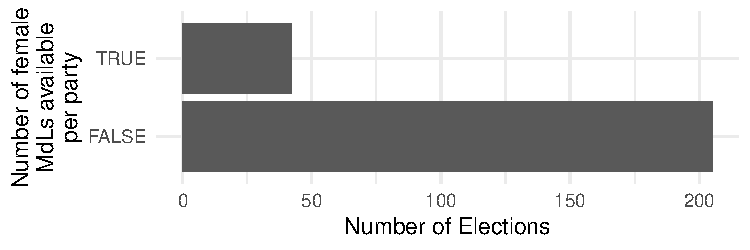
\includegraphics[width = \linewidth]{cbelec/fpsaplot.pdf}
\end{minipage}


\end{longtable}

\begin{longtable}{p{3.2cm}| p{11cm}}
\texttt{total\_female\_
mps\_parliament} &\textbf{Number of Female MPs in Parliament}\newline 
Number of newly elected female MPs.

\hspace*{.25cm}
\begin{minipage}[t]{\linewidth }
\vspace{0pt}
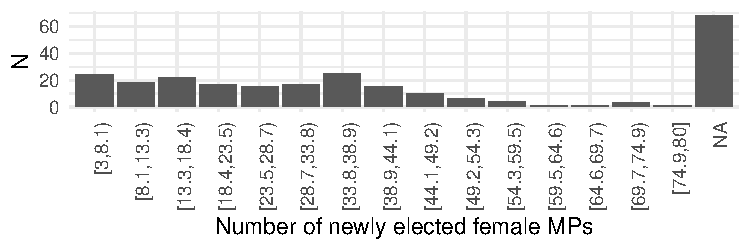
\includegraphics[width = \linewidth]{cbelec/totfemmpsplot.pdf}
\end{minipage}


\end{longtable}

\begin{longtable}{p{3.2cm}| p{11cm}}
\texttt{partyname\_short} &\textbf{Abbreviated Party Name}\newline 
Harmonized abbreviation of the party's name. 372 unique parties.
\end{longtable}

\begin{longtable}{p{3.2cm}| p{11cm}}
\texttt{partyname} &\textbf{Party Name}\newline 
Harmonized name of the party. 372 unique parties.
\end{longtable}

\begin{longtable}{p{3.2cm}| p{11cm}}
\texttt{partyname\_short\_
bundeswahlleiter} &\textbf{Party Name Abbreviation from Bundeswahlleiter}\newline 
Partyname abbreviation as documented by the Bundeswahlleiter. 459 different abbreviations.
\end{longtable}

\begin{longtable}{p{3.2cm}| p{11cm}}
\texttt{partyname\_
bundeswahlleiter} &\textbf{Party Name from Bundeswahlleiter}\newline 
Partyname as documented by the Bundeswahlleiter. 495 different names.
\end{longtable}

\begin{longtable}{p{3.2cm}| p{11cm}}
\texttt{party\_vote\_count} &\textbf{Party Vote Count}\newline 
Number of votes recieved by the party.

\hspace*{.25cm}
\begin{minipage}[t]{\linewidth }
\vspace{0pt}
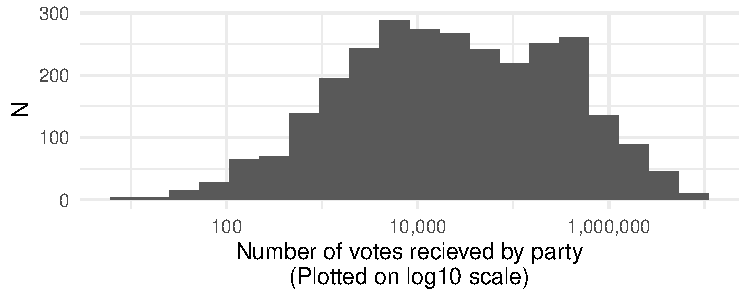
\includegraphics[width = \linewidth]{cbelec/pvcplot.pdf}
\end{minipage}


\end{longtable}

\begin{longtable}{p{3.2cm}| p{11cm}}
\texttt{party\_vshare} &\textbf{Party Vote Share}\newline 
Share of votes recieved by the party.

\hspace*{.25cm}
\begin{minipage}[t]{\linewidth }
\vspace{0pt}
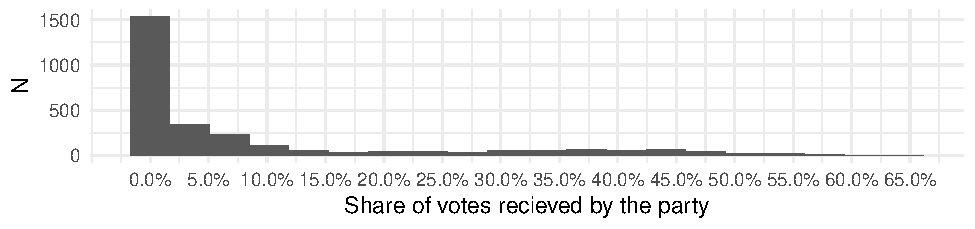
\includegraphics[width = \linewidth]{cbelec/pvsplot.pdf}
\end{minipage}


\end{longtable}

\begin{longtable}{p{3.2cm}| p{11cm}}
\texttt{party\_seat\_count} &\textbf{Party Seat Count}\newline 
Number of seats recieved by the party.

\hspace*{.25cm}
\begin{minipage}[t]{\linewidth }
\vspace{0pt}
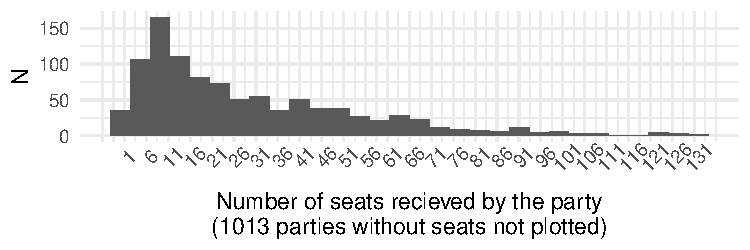
\includegraphics[width = \linewidth]{cbelec/pscplot.pdf}
\end{minipage}


\end{longtable}

\begin{longtable}{p{3.2cm}| p{11cm}}
\texttt{party\_sshare} &\textbf{Party Seat Share}\newline 
Share of seats recieved by the party.

\hspace*{.25cm}
\begin{minipage}[t]{\linewidth }
\vspace{0pt}
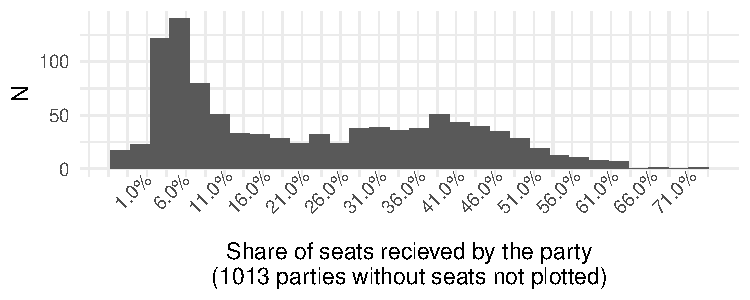
\includegraphics[width = \linewidth]{cbelec/pssplot.pdf}
\end{minipage}


\end{longtable}

\begin{longtable}{p{3.2cm}| p{11cm}}
\texttt{party\_female\_mps} &\textbf{Number of female MPs from party}\newline 
Number of female MPs elected for the party. Note that for parties not elected to the new Landtag party\_female\_mps always is.na() == TRUE.

\hspace*{.25cm}
\begin{minipage}[t]{\linewidth }
\vspace{0pt}
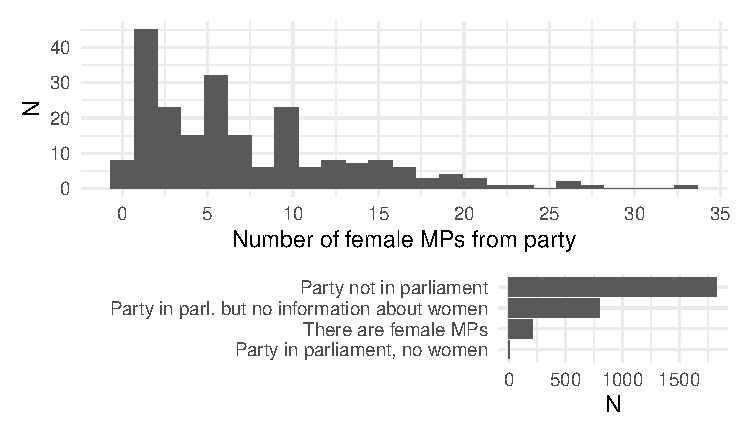
\includegraphics[width = \linewidth]{cbelec/pfmpcplot.pdf}
\end{minipage}


\end{longtable}

\begin{longtable}{p{3.2cm}| p{11cm}}
\texttt{wzb\_govelec\_id} &\textbf{WZB DD GovElec ID}\newline 
If available, MR-Code of the party in the internal govelec database of the WZB department Democracy and Democratization.


\hspace*{.25cm}
\begin{minipage}[t]{\linewidth }
\vspace{0pt}
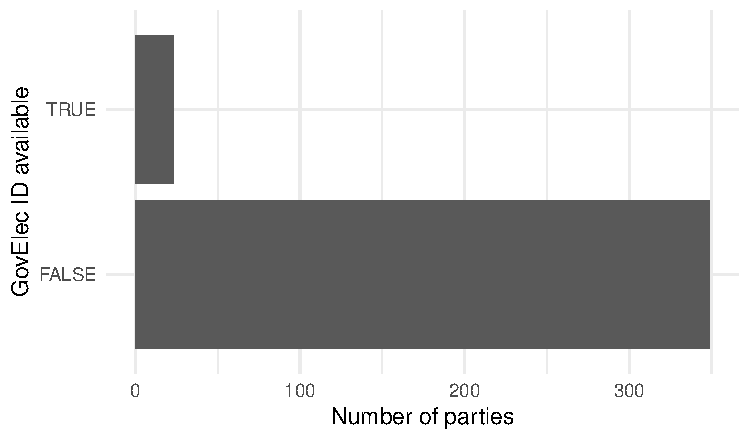
\includegraphics[width = \linewidth]{cbelec/govelecplot.pdf}
\end{minipage}


\end{longtable}

\begin{longtable}{p{3.2cm}| p{11cm}}
\texttt{ches\_id} &\textbf{CHES ID}\newline 
If available, ID of the party in the Chapel-Hill Expert Survey.


\hspace*{.25cm}
\begin{minipage}[t]{\linewidth }
\vspace{0pt}
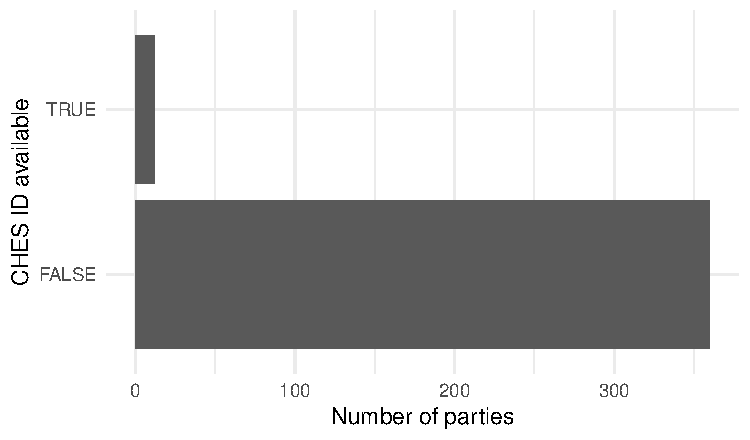
\includegraphics[width = \linewidth]{cbelec/chesplot.pdf}
\end{minipage}



\end{longtable}

\begin{longtable}{p{3.2cm}| p{11cm}}
\texttt{partyfacts\_id} &\textbf{PartyFacts ID}\newline 
If available, ID of the party in the partyfacts database.

\hspace*{.25cm}
\begin{minipage}[t]{\linewidth }
\vspace{0pt}
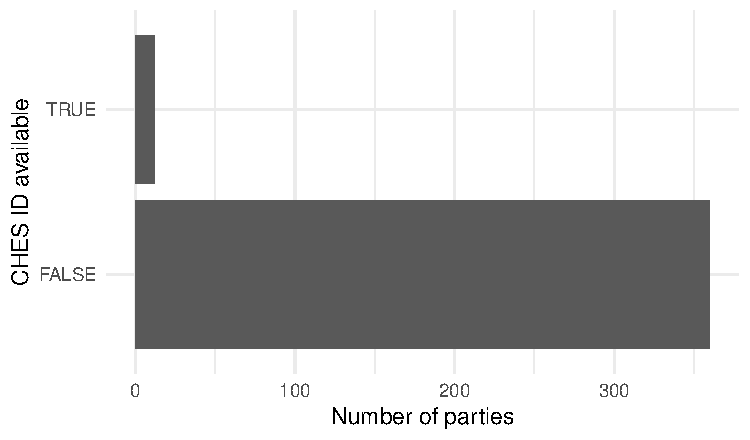
\includegraphics[width = \linewidth]{cbelec/partyfactsplot.pdf}
\end{minipage}



\end{longtable}

\begin{longtable}{p{3.2cm}| p{11cm}}
\texttt{decker\_neu} &\textbf{Chapter Parteienhandbuch}\newline 
Denotes, wether the Handbuch der deutschen Parteien (3. ed.) by Decker and Neu has a chapter on the party.

\hspace*{.25cm}
\begin{minipage}[t]{\linewidth }
\vspace{0pt}
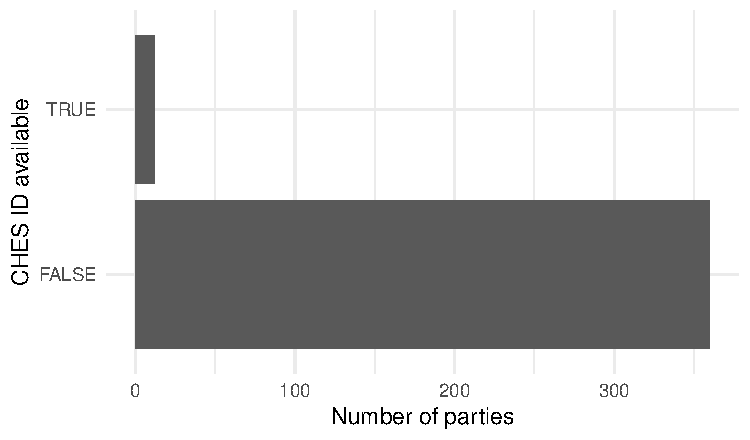
\includegraphics[width = \linewidth]{cbelec/deckerneuplot.pdf}
\end{minipage}



\end{longtable}

\begin{longtable}{p{3.2cm}| p{11cm}}
\texttt{url\_info} &\textbf{URL with additional info on the party}\newline 
URL to informaton on the party on the web. Can contain multiple URLs!
\end{longtable}

\begin{longtable}{p{3.2cm}| p{11cm}}
\texttt{party\_remarks\_
stelzle} &\textbf{Party remarks Stelzle}\newline 
Remarks on the party by me.
\end{longtable}

\begin{longtable}{p{3.2cm}| p{11cm}}
\texttt{party\_remarks\_
bundeswahlleiter} &\textbf{Party remarks Bundeswahlleiter}\newline 
Remarks on the party as listed by the Bundeswahlleiter.
\end{longtable}

\begin{longtable}{p{3.2cm}| p{11cm}}
\texttt{gueltige\_stimm
-zettel\_hh\_hb} &\textbf{Gültige Stimmzettel HH and HB}\newline 
Messy totals.
\end{longtable}

\begin{longtable}{p{3.2cm}| p{11cm}}
\texttt{gesamtstimmen\_by} &\textbf{Gesamtstimmen BY}\newline 
Messy totals.
\end{longtable}

\begin{longtable}{p{3.2cm}| p{11cm}}
\texttt{ausgefallene\_
stimmen\_be} &\textbf{Ausgefallene Stimmen BE}\newline 
Messy totals.
\end{longtable}

\begin{longtable}{p{3.2cm}| p{11cm}}
\texttt{abgegebene\_
stimmen\_hh} &\textbf{Abgegebene Stimmen HH}\newline 
Messy totals.
\end{longtable}

\begin{longtable}{p{3.2cm}| p{11cm}}
\texttt{ungueltige\_
stimmen\_except\_
hh\_hb} &\textbf{Ungültige Stimmen except in HH and HB}\newline 
Messy totals.
\end{longtable}

\begin{longtable}{p{3.2cm}| p{11cm}}
\texttt{ungueltige\_
stimmzettel\_hh\_hb} &\textbf{Ungültige Stimmzettel in HH and HB}\newline 
Messy totals.
\end{longtable}

\end{document}
